\documentclass[spanish,letterpaper,oneside]{article}

\def\documenttitle {Trabajo Final: Una habilidad, un PDA, cinco minutos}
\def\documentsubtitle {Temas selectos de matemáticas I · Cohorte SD26}
\def\documentsubject {Actividad 6 (Sesión 13) · Video Didáctico y Modelación en GeoGebra}
\def\documentauthor {Mtro. Martín Jonathan de la Cruz Muñoz}
\def\coursename {Temas selectos de matemáticas I}
\def\coursecode {PFM02}

\def\universityname {Instituto de Investigación, Innovación y Estudios de Posgrado para la Educación del Estado de Nuevo León}
\def\universityfaculty {Maestría en Aprendizaje y Enseñanza de las Matemáticas}
\def\universitydepartment {Temas selectos de matemáticas I}
\def\universitydepartmentimage {img/iiiepe/marca-iiiepe.png}
\def\universitydepartmentimagecfg {height=1.75cm}
\def\universitylocation {Monterrey, Nuevo León}
\def\studentfullname {Mtro. Martín Jonathan de la Cruz Muñoz}
\def\studentid {00874}
\def\studentemail {martin.delacruz@campus.iiiepe.edu.mx}
\def\programperiod {2do periodo, agosto--noviembre de 2026 (SD26)}
\def\programmodality {Modalidad presencial y en línea}
\def\programshort {MAEM}

\def\authortable {
  \begin{tabular}{ll}
    \textbf{Alumno:} & \studentfullname \\
    Matrícula: & \studentid \\
    Correo institucional: & \studentemail \\
    Unidad: & \coursename \\
    Programa: & \programshort \\
    Periodo: & \programperiod \\
    & \\
    \multicolumn{2}{l}{Fecha de realización: 14 de noviembre de 2026} \\
    \multicolumn{2}{l}{\universitylocation}
  \end{tabular}
}

\input{template}

\usepackage{helvet}
\renewcommand{\familydefault}{\sfdefault}
\usepackage{amsmath,amssymb,booktabs,array,longtable,pdflscape,tikz,tabularx,colortbl,pgfplots,enumitem,needspace}
\usepackage[most]{tcolorbox}
\usetikzlibrary{arrows.meta,positioning,calc,fit,backgrounds,babel}
\pgfplotsset{compat=1.18}

\definecolor{iiiepeNavy}{HTML}{163B5C}
\definecolor{iiiepeBlue}{HTML}{1F6F9F}
\definecolor{iiiepeAqua}{HTML}{20B7A8}
\definecolor{iiiepeOrange}{HTML}{F28C28}
\definecolor{iiiepePaper}{HTML}{F6F8F7}
\definecolor{iiiepeInk}{HTML}{1E2A32}
\definecolor{iiiepePale}{HTML}{EEF5F8}
\def\portraittitlecolor {iiiepeNavy}
\setcitestyle{authoryear,open={(},close={)}}

\newcommand{\insertcoverwatermark}{%
  \AddToShipoutPictureBG*{%
    \begin{tikzpicture}[remember picture,overlay]
      \node[opacity=.06,inner sep=0pt] at (current page.center)
      {
\includegraphics[width=.58\paperwidth]{img/iiiepe/logo-puntos.png}};
    \end{tikzpicture}%
  }%
}

\newtcolorbox{propuestabox}[1][]{%
  enhanced,breakable,
  colback=iiiepePaper,colframe=iiiepeAqua!80!iiiepeNavy,
  boxrule=1pt,leftrule=4pt,arc=2pt,
  left=8pt,right=8pt,top=6pt,bottom=6pt,
  before skip=6pt,after skip=10pt,
  fonttitle=\bfseries\color{white},coltitle=white,
  colbacktitle=iiiepeNavy,
  attach boxed title to top left={xshift=8pt,yshift=-2pt},
  boxed title style={colback=iiiepeNavy,colframe=iiiepeNavy,arc=1pt},
  title={Propuesta didáctica},#1}

\setlength{\parskip}{5pt}\setlength{\parindent}{0pt}
\begin{document}\insertcoverwatermark\templatePortrait\templatePagecfg\templateFinalcfg\fancyfoot{}\fancyfoot[L]{\scriptsize IIIEPE · MAEM · SD26}\fancyfoot[C]{\scriptsize\thepage}\fancyfoot[R]{\scriptsize Actividad 6}\setstretch{1.25}\raggedbottom

\section{Síntesis del Trabajo Final y vinculación curricular}
El Trabajo Final de \textit{Temas Selectos de Matemáticas I} plantea la producción de un video didáctico de entre cuatro y cinco minutos para retomar y profundizar la propuesta de la Sesión 12 \citep{iiiepe2026_s13}. En esta entrega se desarrolla la \textbf{variación directamente proporcional en sistemas hidráulicos} ($F_2 = k\cdot F_1$), articulando las ocho habilidades matemáticas de la SEP \citep{sep1994} con énfasis explícito en \textbf{Generalizar} (en sinergia con \textit{Inferir} y \textit{Comunicar}) y el Proceso de Desarrollo de Aprendizaje (PDA) correspondiente al Bachillerato Tecnológico CONALEP dentro del Marco Curricular Común \citep{sep2023_mccems}.

\begin{enumerate}
  \item \textbf{Habilidad matemática SEP:} \textit{Generalizar} (en sinergia con \textit{Inferir} y \textit{Comunicar}): descubrir regularidades en datos experimentales y geométricos para formular la regla algebraica general $y = k x$, interpretando $k$ como ventaja mecánica y extrapolando el modelo a nuevas condiciones.
  \item \textbf{Contenido disciplinar:} Principio de Pascal en fluido incompresible confinado, en equilibrio hidrostático cuasiestático y sin pérdidas por fricción, junto con la variación proporcional directa en prensas y actuadores hidráulicos:
  \[
    P_1 = P_2 \implies \frac{F_1}{A_1} = \frac{F_2}{A_2} \implies F_2 = \left(\frac{A_2}{A_1}\right) F_1 = \left(\frac{d_2}{d_1}\right)^2 F_1 = k\cdot F_1.
  \]
  \item \textbf{PDA SEP:} Articula \textit{Saberes y Pensamiento Científico} con \textit{Pensamiento Matemático} \citep{sep2023_mccems}: el estudiante resuelve problemas de variación proporcional directa en contextos de física e ingeniería, representando la relación fuerza--área mediante tablas, expresión algebraica y gráfica lineal en GeoGebra, e interpretando $k$ como factor de amplificación.
\end{enumerate}

\section{Explicación matemática, dificultad frecuente, estrategia y reto}
Al comparar dos jeringas o pistones cilíndricos con diámetros $d_1 = 1.5\text{ cm}$ y $d_2 = 3.0\text{ cm}$, la razón lineal de diámetros es $d_2/d_1 = 2$; sin embargo, dado que el área transversal circular ($A = \pi d^2/4$) depende cuadráticamente del diámetro, el factor de amplificación resulta:
\[
  k = \frac{A_2}{A_1} = \left(\frac{d_2}{d_1}\right)^2 = \left(\frac{3.0}{1.5}\right)^2 = 2^2 = 4.
\]
Para el pistón de entrada de área $A_1 = \pi (1.5\text{ cm})^2 / 4 \approx 1.767\text{ cm}^2$ sometido a una fuerza aplicada $F_1 = 8\text{ N}$, la presión confinada resulta $P = F_1/A_1 \approx 4.53\text{ N/cm}^2$ ($45\,270\text{ Pa}$), por lo que la fuerza de salida alcanza $F_2 = 4(8\text{ N}) = 32\text{ N}$. Es decir, dependiendo del diseño, si $k > 1$ hay amplificación de fuerza, si $k = 1$ la transmisión es directa y, en cambio, si $k < 1$ se reduce fuerza ganando recorrido. Por conservación del volumen de fluido ($A_1\Delta x_1 = A_2\Delta x_2$) y del trabajo mecánico ideal, se verifica:
\[
  W_1 = F_1\,\Delta x_1 = (8\text{ N})(0.04\text{ m}) = 0.32\text{ J}, \qquad W_2 = F_2\,\Delta x_2 = (32\text{ N})(0.01\text{ m}) = 0.32\text{ J},
\]
por lo que, cuando el émbolo menor recorre $\Delta x_1 = 4\text{ cm}$, el émbolo mayor se desplaza $\Delta x_2 = \Delta x_1 / k = 4/4 = 1\text{ cm}$.

\textbf{Dificultad frecuente del alumnado y remediación:} El error habitual consiste en usar directamente la razón lineal de diámetros ($k = d_2/d_1 = 2$) sin elevar al cuadrado, obteniendo erróneamente $F_2 = 2(8\text{ N}) = 16\text{ N}$ en lugar de $32\text{ N}$, lo que representa una subestimación de $-16\text{ N}$ ($50\,\text{\symbol{37}}$ de error). Este obstáculo cognitivo surge al no coordinar el registro numérico con el geométrico \citep{duval2006}; por ello, en el video se deriva explícitamente el área circular mostrando cómo $\pi/4$ se cancela en el cociente y se contrastan las rectas real ($F_2 = 4F_1$) y errónea ($F_2 = 2F_1$) en GeoGebra Classic:

\begin{figure}[htbp]
\centering
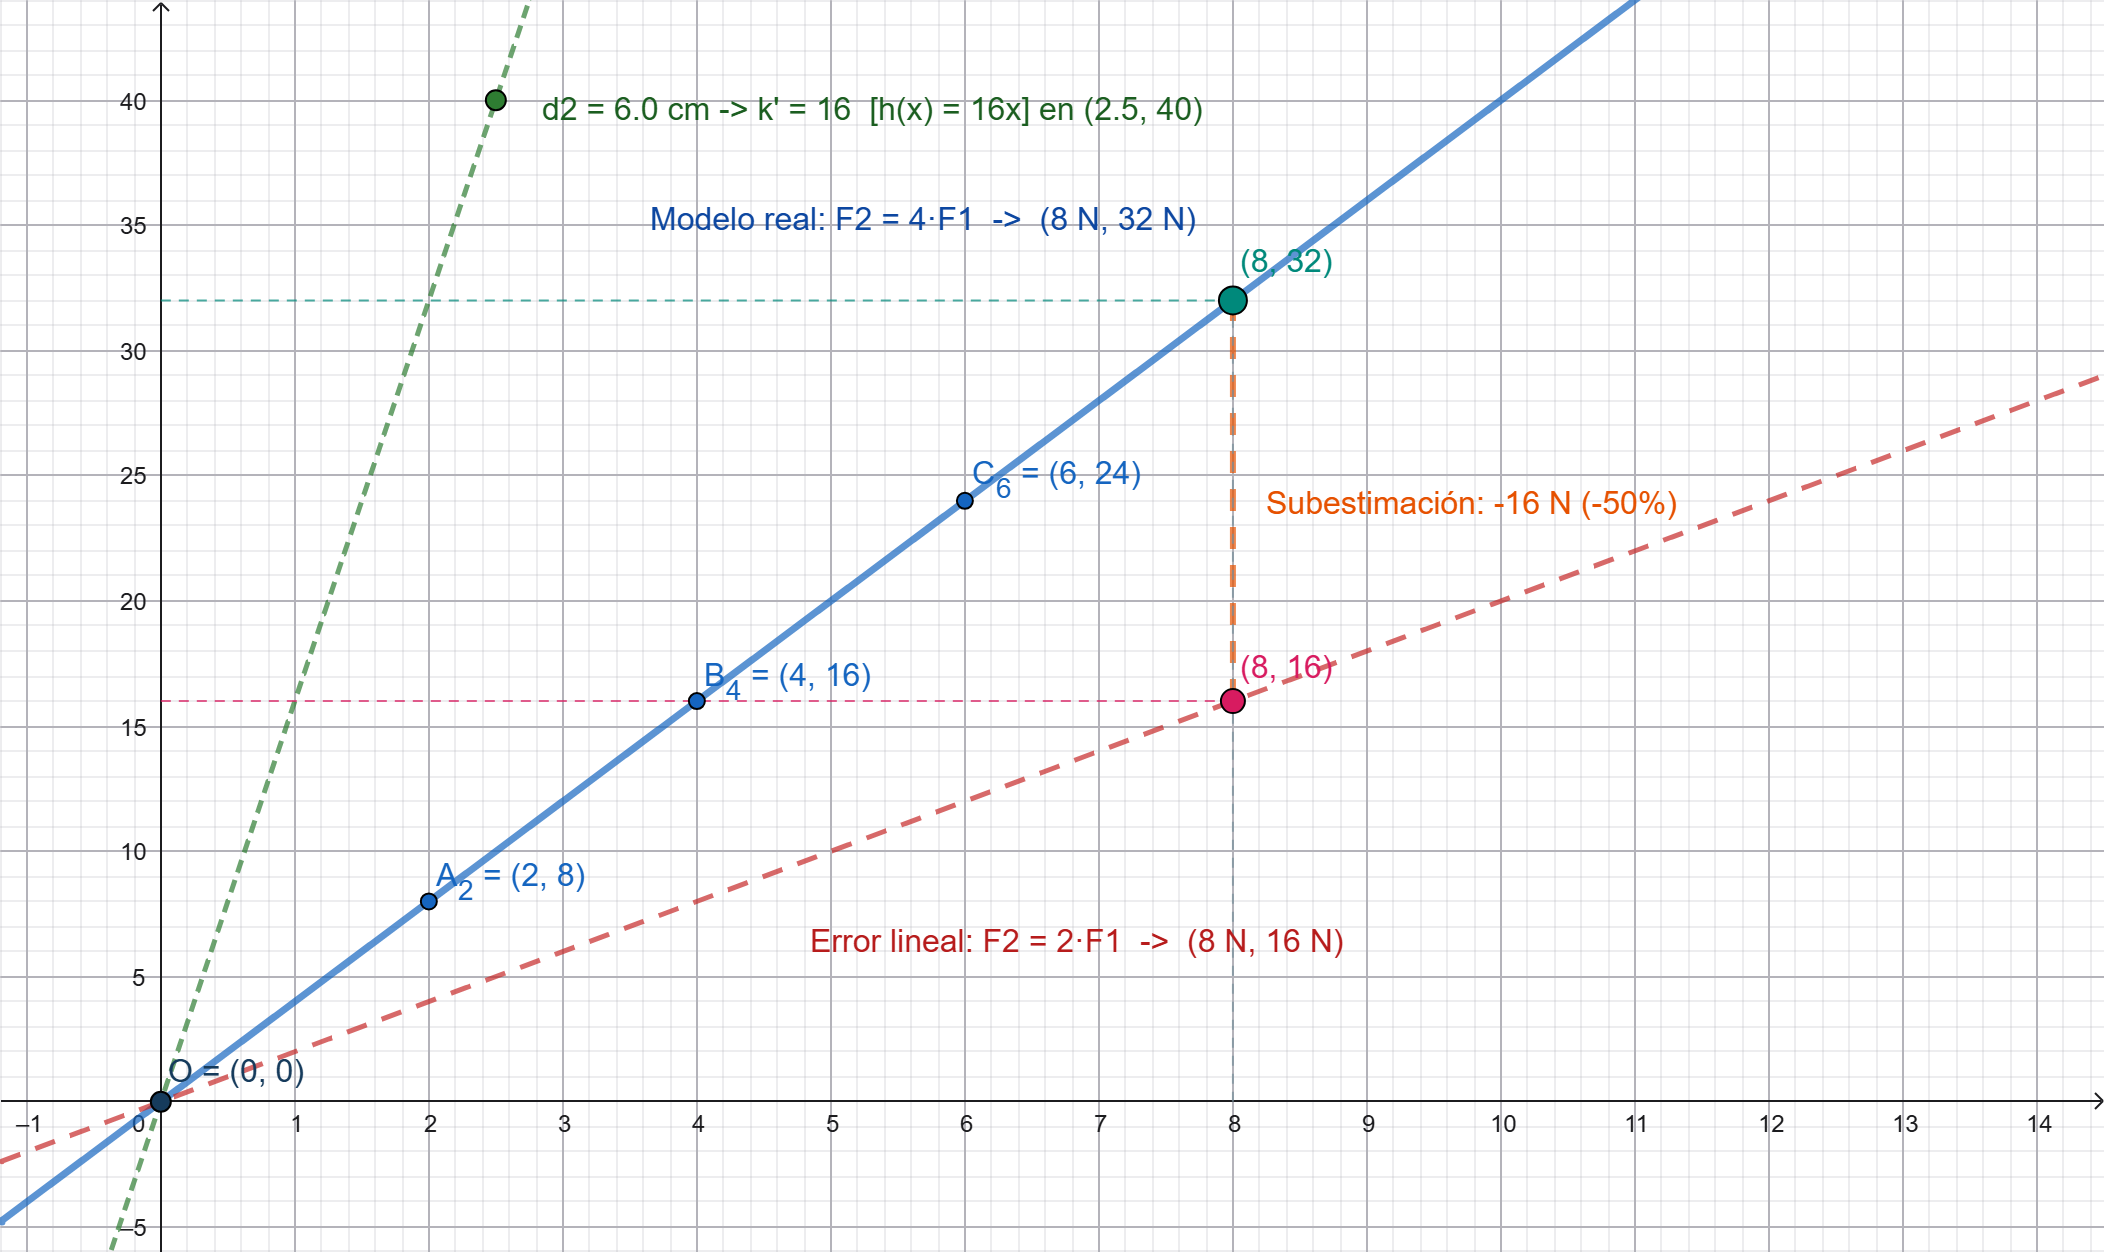
\includegraphics[width=0.86\linewidth]{img/geogebra/act6_video_32N.png}
\caption{Modelación en GeoGebra Classic: modelo real $F_2 = 4 F_1$ pasando por $(8\text{ N}, 32\text{ N})$, error lineal $F_2 = 2 F_1$ en $(8\text{ N}, 16\text{ N})$ con subestimación de $-16\text{ N}$ ($-50\,\text{\symbol{37}}$) y extensión cuadrática $F_2 = 16 F_1$ para $d_2 = 6.0\text{ cm}$.}
\end{figure}

\textbf{Estrategia didáctica para la enseñanza y el aprendizaje:} La secuencia articula la resolución de problemas y las fases heurísticas de \citet{polya1945} con estrategias de las \textit{Cien Técnicas Didácticas} \citep{unadm_tecnicas} orientadas al desempeño activo del estudiante:
\begin{itemize}
  \item \textbf{Proyectos colaborativos (UnADM \#96) y Heurística de Bruner (UnADM \#69):} Construcción y exploración empírica del brazo hidráulico con dos jeringas ($d_1 = 1.5\text{ cm}$, $d_2 = 3.0\text{ cm}$) conectadas por manguera con fluido, registrando fuerzas y recorridos en tabla experimental.
  \item \textbf{Autoexplicación (UnADM \#16):} Contrastación argumentada entre la predicción intuitiva lineal ($k = 2 \Rightarrow 16\text{ N}$) y la razón cuadrática del área ($k = 4 \Rightarrow 32\text{ N}$) para verbalizar por qué duplicar el diámetro cuadruplica la fuerza.
  \item \textbf{Simulación interactiva (UnADM \#99):} Verificación de la pendiente $k$ y la conservación $F_1 \Delta x_1 = F_2 \Delta x_2$ en GeoGebra Classic, observando en tiempo real el efecto de variar $d_2$.
  \item \textbf{Estudio intercalado (UnADM \#40):} Aplicación graduada en el reto matemático de cuatro incisos combinando cálculo numérico, análisis inverso del desplazamiento y generalización algebraica.
\end{itemize}

\textbf{Reto matemático planteado en el video:} \textit{``En un brazo excavador construido con jeringas hidráulicas ($d_1 = 1.5\text{ cm}$, $d_2 = 3.0\text{ cm}$, $F_1 = 8\text{ N}$ y recorrido $\Delta x_1 = 4\text{ cm}$), (a) calcula la presión $P$ en el fluido y (b) la fuerza real $F_2$ aplicando Heurística de Bruner (\#69) y Autoexplicación (\#16); (c) determina el desplazamiento $\Delta x_2$ del émbolo receptor; y (d) ejercita la habilidad SEP de Generalizar deduciendo qué sucede con $k$ y la pendiente si el diámetro receptor se duplica hasta $d_2 = 6.0\text{ cm}$ ($k' = (6/1.5)^2 = 16$, $F_2 = 16 F_1 = 128\text{ N}$)''.} El video incluye una pausa cognitiva de $15\text{ s}$ (\texttt{03:40--03:55}) para que el estudiante resuelva los incisos antes de la comprobación paso a paso ($P \approx 4.53\text{ N/cm}^2$, $F_2 = 32\text{ N}$, $\Delta x_2 = 1\text{ cm}$ y $k'=16$).

\textbf{Indicador y evidencia observable:} El alumno formula la ecuación $F_2 = k\cdot F_1$ con $k = (d_2/d_1)^2$ correcto y calcula $\Delta x_2 = \Delta x_1 / k$; su desempeño se constata mediante (1) tabla de valores, (2) gráfica con pendiente en GeoGebra Classic y (3) respuesta escrita argumentada al inciso (d).

\section{Recursos audiovisuales y alineación con los 9 criterios de la rúbrica}
El producto audiovisual integra diagramación animada de ecuaciones y gráficas de GeoGebra Classic, narración didáctica clara en español, audio maestro de $48\text{ kHz}$ y subtítulos sincronizados en formato externo \texttt{.srt} sin incrustar sobre la imagen, garantizando la lectura limpia de expresiones y gráficas:
\begin{itemize}
  \item \textbf{Video MP4 (versión limpia sin subtítulos incrustados):} \texttt{video-alternativo-visual-sin-subtitulos-temas-selectos-matematicas-i-SD26-act-06-trabajo-final\_Martin-Jonathan-de-la-Cruz-Munoz.mp4} ($1280\times 720$, $24\text{ fps}$, duración exacta \textbf{4:46 min / 286.71 s}, dentro del intervalo oficial de 4:00 a 5:00 min).
  \item \textbf{Enlace público del video en YouTube:} \url{https://youtu.be/xZOLQRSTyQE}
  \item \textbf{Respaldo del video MP4 en Google Drive:} \url{https://drive.google.com/file/d/1ymyhV10cpDZcRXstzPY6XJKAvsH4Z8TJ/view?usp=sharing}
  \item \textbf{Subtítulos sincronizados (\texttt{.srt}, 33 líneas) en Google Drive:} \url{https://drive.google.com/file/d/1jCVriFoGUnHOuNbjm8x-xL6qCkxLQWcc/view?usp=sharing}
  \item \textbf{Documentación complementaria:} Guion editable en Word (\texttt{Guion Trabajo Final}), presentación visual 16:10 y reporte técnico alineado a la propuesta de la Sesión 12.
\end{itemize}

{\small\setstretch{1.05}\renewcommand{\arraystretch}{1.10}
\begin{longtable}{|>{\raggedright\arraybackslash}p{0.27\linewidth}|>{\centering\arraybackslash}p{0.16\linewidth}|>{\raggedright\arraybackslash}p{0.53\linewidth}|}\hline
\rowcolor{iiiepePale} \textbf{Criterio de la Rúbrica} & \textbf{Bloque y tiempo} & \textbf{Evidencia en el Video y Documentación} \\\hline
\endfirsthead\hline
\rowcolor{iiiepePale} \textbf{Criterio de la Rúbrica} & \textbf{Bloque y tiempo} & \textbf{Evidencia en el Video y Documentación} \\\hline
\endhead
1. Vinculación habilidad, contenido y PDA & Bloque 1 (0:22--1:14) & Expone las 8 habilidades SEP, centra la habilidad \textit{Generalizar} (con \textit{Inferir} y \textit{Comunicar}), el contenido $F_2=k\cdot F_1$ y el PDA completo. \\\hline
2. Explicación matemática & Bloque 2 (1:14--2:22) & Derivación del Principio de Pascal, cociente de áreas $(d_2/d_1)^2$, regímenes de $k$ y conservación $\Delta x_2=\Delta x_1/k$. \\\hline
3. Dificultades frecuentes & Bloque 3 (2:22--2:48) & Contraste numérico y gráfico entre error lineal ($k=2 \Rightarrow 16\text{ N}$) y real ($k=4 \Rightarrow 32\text{ N}$, $-50\,\text{\symbol{37}}$) con cancelación de $\pi/4$. \\\hline
4. Estrategia didáctica y recursos & Bloque 4 (2:49--3:12) & Articula SEP y Pólya con técnicas UnADM: Proyectos colaborativos (\#96), Heurística de Bruner (\#69), Autoexplicación (\#16) y Simulación en GeoGebra (\#99). \\\hline
5. Reto matemático & Bloque 5 (3:13--4:20) & Reto de excavadora hidráulica con Estudio intercalado (\#40), pausa activa (3:40--3:55) y comprobación de los 4 incisos hasta $d_2=6\text{ cm}$ ($k'=16$). \\\hline
6. Indicador y evidencia observable & Bloque 6 (4:20--4:32) & Indicador de formulación algebraica/desplazamiento y evidencia en tabla, gráfica GeoGebra y respuesta escrita del inciso (d). \\\hline
7. Creatividad e innovación & Todo el video (0:00--4:46) & Esquemas animados en corte hidráulico, pausa cognitiva cronometrada, gráfica comparativa en GeoGebra y prototipo experimental. \\\hline
8. Calidad y organización audiovisual & Todo el video (0:00--4:46) & Video HD $1280\times 720$ limpio sin texto obstruido, audio maestro $48\text{ kHz}$ y archivo externo \texttt{.srt} sincronizado. \\\hline
9. Duración y tiempo & Cierre (4:32--4:46) & \textbf{4:46 min} ($286.71\text{ s}$), equilibrio temporal entre los 6 bloques dentro del rango oficial de $4:00$ a $5:00\text{ min}$. \\\hline
\end{longtable}}

\needspace{5\baselineskip}\section*{Referencias}
{\setstretch{1.15}\setlength{\parskip}{6pt}
\par\hangindent=1.27cm\hangafter=1 Instituto de Investigación, Innovación y Estudios de Posgrado para la Educación del Estado de Nuevo León. (2026). \textit{Actividad 6. Trabajo Final: Una habilidad, un PDA, cinco minutos (Guión y rúbrica oficial)}. EVA Posgrados IIIEPE.
\par\hangindent=1.27cm\hangafter=1 Secretaría de Educación Pública. (1994). \textit{Libro para el maestro. Matemáticas. Educación secundaria}. SEP.
\par\hangindent=1.27cm\hangafter=1 Secretaría de Educación Pública. (2023). \textit{Marco Curricular Común de la Educación Media Superior (MCCEMS): Pensamiento Matemático}. SEP.
\par\hangindent=1.27cm\hangafter=1 Universidad Abierta y a Distancia de México. (s.f.). \textit{Cien técnicas didácticas para la enseñanza y el aprendizaje en entornos educativos}. UnADM.
}

\end{document}
